 

%\subsection{Dynamic Simulation}
%In order to comment on safety performance the simulated dynamics of the AGV a custom simulation was deveoped in Python. There is a great deal of software already available for simulating vehicle interactions. We reviewed those discussed below, but found it was more approporiate to further develop the simulation used for our earlier work to answer research questions related to the operation of robotic intralogistics vehicles \cite{Lambert2020a}.
%
%These additional dynamic effects mean the timing specification sent by the intersection controller will always be missed by a small amount as it would be if the controller was communicating with embodied robots acting in a real logistics environment. In order to comment on the total energy consumption, it would be useful to model second order dynamics, allowing the dissipated power to be approximated by the acceleration. Acceleration is a good proxy for motor power in a low speed system like logistics, where there is little air resistance but lots of stopping and starting. In order to investigate the effect of communication latency the simulation time-step should be smaller than the hypothetical communication latency for client/server control over a limited bandwidth network. Lateral tracking behaviour need not be considered if we assume all AGV are able to traverse the given path with negligible lateral error. This is not too unrealistic if the paths account for dynamic limitations limitations of the vehicles which will traverse them such as radial polynomials \cite{Digani2014obs} or clothoid transitions \cite{lambertoptimalobstacles}.
%
%With these requirements in mind, a number of off-the-shelf traffic simulation software packages were investigated. To give a brief overview we considered traditional closed source modelling software such as DRACULA \cite{Liu2005}, MATSim \cite{AndreasHorni2016}, PTV VISSIM \cite{Kara2014} and Aimsun \cite{lenorzer2015modelling}. These are powerful tools with a focus on recreating interesting microscopic traffic behaviour arising from human driven vehicles. For example DRACULA operates on a detailed road network combined with trip matrix indicating travel demand. Vehicles enter the network according to a distribution which corresponds to the trip matrix. Individual vehicles are tracked until they reach their destination, as if they parked off the road. Average speeds are calculated based on completed trips making it possible to comment on the expected delay for a journey which began at a certain time. Different junction types with and without traffic lights are handled with custom logic and are inherently conflict-free. Longitudinal behaviour is based on the intelligent driver model of human car following which is more realistic than the earlier Gipps model, but still cannot guarantees that a safe distance will be maintained within the dynamic limitations of the vehicles, which is required to guarantee collision avoidance. SUMO \cite{Busquets2016}, is an open source traffic simulator also intended as a model of human operated vehicles. It is highly configurable, and with enough modification it would be possible to modify both the  individual vehicle logitudinal control and the intersection control to reflect the two -layer control architecture proposed by \cite{Digani2015} but the only components then reused would be the vehicle dynamcs, the position trackjing and the vizualization. The tool for generating large pattern based roadmaps based on grids or webs could be used standalone, according to the open `.net' format, based on `.xml'
%
%Another option considered was using an existing robot dynamic simulator. Stage \cite{Vaughan2008} is designed for large numbers of robots, but is unsuitable as it relies on a first order dynamics. Another option was Gazebo \cite{Rivera2019} which has been used in similar works such as \cite{Walenta2017} and \cite{Yan2017}, where ROS (Robot Operating System) libraries were used to implement the control algorithms, so the same binaries could equally be linked to a full Gazebo simulation or a collection of physical test robots. This is a great option but would force us to implement robust lateral control and other systems needed for a real AGV which are incidental to our contribution. %In \cite{Digani2019}, leveraged an industrial partner to fill this gap. 
%ROS1 also has some issues with multiple vehicles which require another system to work around, for example another library Fawkes in one notable competition \cite{Niemueller2017}. An better option would be the new ROS2 library which does away with the single master architecture and TCP messaging protocol \cite{Eros2019} but is more sparsely documented and under active development at the time of writing, so we leave it for further work. 
%
%%Initial experiments reported in \cite{Lambert2020a} and \cite{Lambert2020b}, made use of a bespoke Python simulation. We continued to develop this custom simulation to add the required functionality, instead of heavily modifying an existing microsimulation package or adding multiple vehicles to a dynamic simulator like Gazebo. The Python files for our simulation, and all the tested controllers are available in GitHub \cite{Lambert2020}.   

\section{Application Context}
\subsection{Roadmap-based AGV System}
Consider a demand responsive AGV system for intra-logistics \cite{Boysen2019} or a smart factory \cite{Dotoli2019}. The system is concerned with completing a series of material transfer tasks. 
%The assumption each task consists of moving one unit load from a given pick location to the specified drop location. 
A well known solution to motion planning in a well known environment involves simplifying the free space into a (possibly irregular) lattice of reachable states, connected by arcs if there exists a feasible transition from one state to the other, to create  roadmap which can be encoded as a graph. A sequence of intermediate positions associated with each arc is sometimes stored alongside to avoid online re-computation. Using the roadmap graph, motion plans between any two states can be generated using a shortest path algorithm, which are detailed enough to be followed by the lateral position controller on board the vehicle. 

In a centralized system the transfer tasks are assigned to available AGVs by a single scheduler which is aware of the status of every task and the position of every vehicle. The optimal assignment would minimize the makespan or total time for the completion of all tasks, but in practice this may be too time consuming, especially if new tasks are being generated all the time like in a fulfilment centre \cite{Azadeh2019}. Conflict-free route planning depends on the task assignment and can be solved for jointly along with the assignment or performed sequentially based on a fixed assignment by searching the space time extended network to guarantee collisions are avoided.

Recently a number of decentralized systems have been developed which offer advantages in the number of vehicles that can operate in one area, reduced downtime for reconfiguration and safe interaction with human operators \cite{Fragapane2021} . In \cite{Walenta2017}, a roadmap representation is still used, but the roadmap is shared between vehicles. The partially decentralized system described in \cite{Digani2014coord} combines traffic routing with per-intersection control is primarily roadmap based. In \cite{Cardarelli2017} is it improved with the possibility for an AGV to deviate from the roadmap based on its own sensors and based on a shared sensor state called the global live view. In such a decentralized system, an intersection controller cannot be assumed to know the motion plan of approaching vehicles, unless they communicate their intention as part of the protocol. To this end it is assumed a channel exists with sufficient bandwidth and a fixed latency $T$ for the messages described in Section \ref{sec:dual_waypoint}.

\section{Modelling Plant and Interacting Digital Control Systems}
To examine the approach to intersection control, we include an agent based model for every AGV at the intersection with access to strictly limited information which might be available from on-board sensors. All additional state information is sent according to the messaging interface defined in Section \ref{sec:dual_waypoint}. It is an implementation of AIM* \cite{Levin2017}, with some adaptations to use the roadmap representation of Digani et al, which is typical in the AGV space \cite{Digani2019}. AIM* was selected as it offers scope for the intersection controller to improve performance through optimization, compared to earlier interface descriptions such as \cite{Dresner2004}.  
\subsection{Dual Waypoint Interface}
\label{sec:dual_waypoint}
The dual waypoint interface is designed to be decoupled from the algorithms for scheduling and routing as far as possible. In order to support decentralized routing with adaptive paths, each approaching vehicle must send an ApproachPlan message to containing a detailed plan for how it intends to cross the intersection.  The ApproachPlan contains four parameters $d =\left[ t_A, \bm{X}( s_A ), v_A, \bm{X}(s) \right]$. The plan consists of a transmission timestamp $t_A$, a measured position $\bm{X}(s_A)$, and speed $v_A$ at the given time and a sequence of feasible positions with no timing information, the path $\bm{X}(s)$. 

Embedding the path in each request for guidance means that approaching AGV can use obstacle avoidance planning before they enter the approach lane, and still receive the correct speeds at the intersection. As a result the size and shape of the conflict zone is not fixed but depends on the current traffic situation and the approach plans received.

The conflict zone shape is calculated by discretizing $\bm{X}(s)$ into linear segments of length $L=1$m and searching for points where the minimum distance between two segments exceeds the diameter of the AGV bounding circle, and the direction of the segment is different. This ensures there is no conflict point identified where one segment joins another, which arises when two AGV are following the same path one after the other.  

The intersection controller is responsible for generating an optimal speed profile for this path $v(t)$, to create a trajectory which satisfies the collision avoidance constraints with the trajectories of all known approaching vehicles $\bm{\xi}_i(t) \forall i \in N$. 

The trajectory across the intersection $\bm{\xi}(t)$ is found from the path $\bm{X}(s)$, the start time $t_A$ and start position $\bm{X}(s_A)$ using Equation \ref{eq:integrate}.
\begin{equation}
\bm{\xi}(t)  = \bm{X}(s_A) + \int_{t_A}^{t_L} \bm{X}\left( v(t) \right)  dt
\label{eq:integrate}
\end{equation}

The speed profile is always expressed as two average speeds for two segments. The first segment $AB$ begins at the position of the AGV at transmission time $\bm{X}(s_A)$, and ends at the nearest edge of the intersection conflict zone $\bm{X}(s_B)$. The second segment $BC$ begins at $\bm{X}(s_B)$ and ends at the far edge of the intersection conflict zone $\bm{X}(s_C)$.  

To represent this level of detail, the DualWaypoint contains four parameters $d =[t_B, t_C, s_B, s_C]$. These are independent of the discretization in the ApproachPlan, and expressed in path coordinates. The flow of messages over time is shown in Figure \ref{fig:dual_wp_message_sequence}.

\begin{figure}[ht]
	\centering
	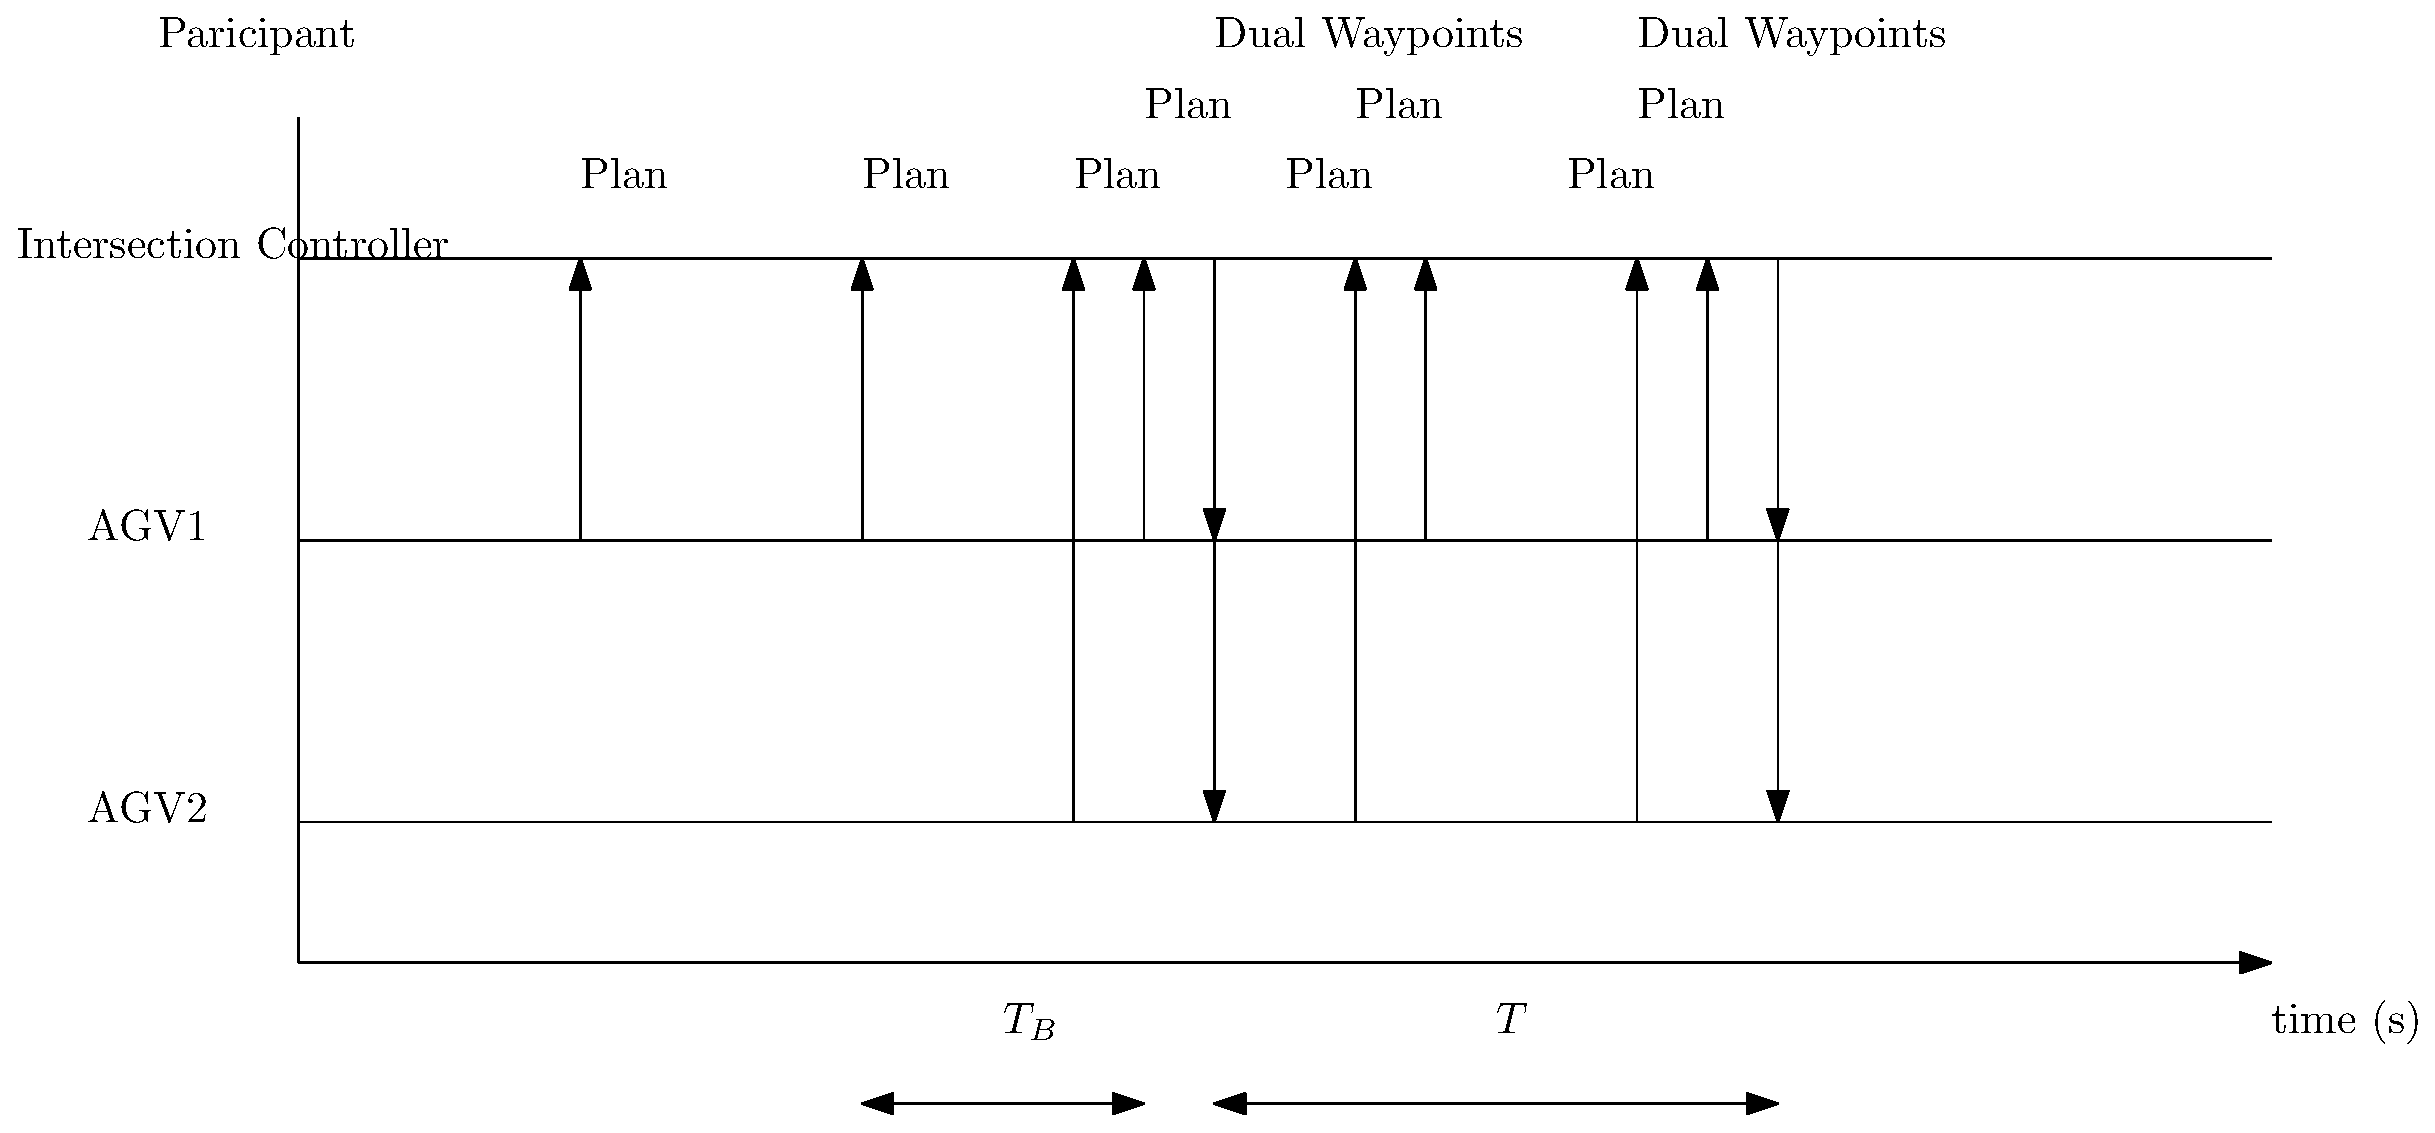
\includegraphics[width=0.9\linewidth]{dual_wp_message_sequence.eps}
	\caption{Sequence diagram for two AGVs communicating with the Intersection Controller which sends a DualWaypoint message to every known AGV every $T$ seconds, considering the latest ApproachPlans it has received to date. }
	\label{fig:dual_wp_message_sequence}
\end{figure}


\subsection{Longitudinal Speed Control}
Longitudinal Speed Control for each Individual AGV is based on two main behaviours. The first one determines the speed on unconflicted links. The second one is required meet the timing specification contained in the Dual Waypoint message, subject to disturbances and uncertainty in the plant using position feedback.  

Previous authors have modelled the speed on unconflicted links using car-following behaviour models. Automated traffic is assumed to follow an Adaptive Cruise Control Model with set headway, while human operated vehicles follow the Intelligent Driver Model in \cite{Baz2020}. In the AGV space it is common to simplify car-following with mutual exclusion of discretized roadmap segments  \cite{Digani2014coord} so we follow this scheme for the main results. Some results with mutual exclusion turned off are given in  in Section \ref{sec:fixed_arrival_pattern} before the main results with mutual exclusion in Section \ref{sec:mutex_arrival_pattern}. The update period $T_L=0.1$s must shorter or equal to that of the intersection controller $T$. 

The Dual Waypoint Timing Specification is met with a constant acceleration model based on the collision-free operation modes in \cite{He2020}. 
Our simulation incorporates two modes, depending on whether the vehicles position feedback $\bm{X}(\hat{s})$ at time $\hat{t}$ indicates it is approaching the conflict zone so $\hat{s}<s_B$ or already inside it so $s_B\leq s_A<s_C$. If the AGV has passed the conflict $\hat{s}>s_C$ then its speed is unconstrained from the perspective of this intersection controller. In the simulation exiting vehicles would accelerate to maximum speed, at $\alpha_{max}$.

On approach to the conflict zone, where $\hat{s}<s_B$, the approach acceleration $\alpha_{AB}$ is given by Equation \ref{eq:approach}.
\begin{equation}
\alpha_{AB} = \frac{(s_B - \hat{s}) - \hat{u}(t_B - \hat{t}) }{0.5 (t_B - \hat{t})^2}
\label{eq:approach}
\end{equation}

Within the conflict zone $s_B \leq s_A<s_C$ the acceleration $\alpha_{BC}$ is given by Equation \ref{eq:within}.
\begin{equation}
\alpha_{BC} = \frac{(s_C - \hat{s}) - \hat{u}(t_C - \hat{t}) }{0.5 (t_C - \hat{t})^2}
\label{eq:within}
\end{equation}

\subsection{AGV Motor Dynamic and Electrical Model}
For the dynamics, every AGV was assumed to have the same mass $M=100$kg whether loaded or unloaded, reflecting a negligible cargo mass, for example spare parts for mobile phone repair. An AGV may be propelled by brushless DC motors, which provide high torque and efficiency. Even so, a major source of power loss is internal resistance of the windings and magnetic losses in the core.  %This is captured in the equivalent circuit with one lumped resistor $R$ shown in Figure \ref{fig:dc_motor}. Suitable parameters for the equivalent circuit are shown in Table \ref{tab:params} and were found in a test of an electric bicycle \cite{Racewicz2018}.
The field strength of the magnets, the number of poles and the number turns of the armature coils can be captured in the motor constant $k_T $ relating torque $\tau$ [Nm] to armature current.

\begin{equation}
\tau = k_T I_a
\label{eq:torque_constant}
\end{equation} 

Similarly, the rotational speed $\omega$ [rpm] is related to the back emf $\epsilon$ [V] by Equation \ref{eq:emf_constant}.

\begin{equation}
\omega = {k_e}\epsilon_D 
\label{eq:emf_constant}
\end{equation}

These can be combined to give the plant model for one AGV in Equation \ref{eq:model}

\begin{equation}
\ddot{x} =\frac{ u \cdot k_T (V_{CC} - \epsilon_D) }{M R_a d_W/2}
\label{eq:model}
\end{equation}

 There are numerous loss sources in an electric motor such as winding resistance, flux leakage, eddy currents in the core and so on \cite{Sarlioglu2016}. By using real-world measured mechanical power output and electrical input, an equivalent winding resistance $R_a$ for the simple model can be found. The parameters are shown in Table \ref{tab:motor_params}.

\begin{figure}[ht]
	\centering
	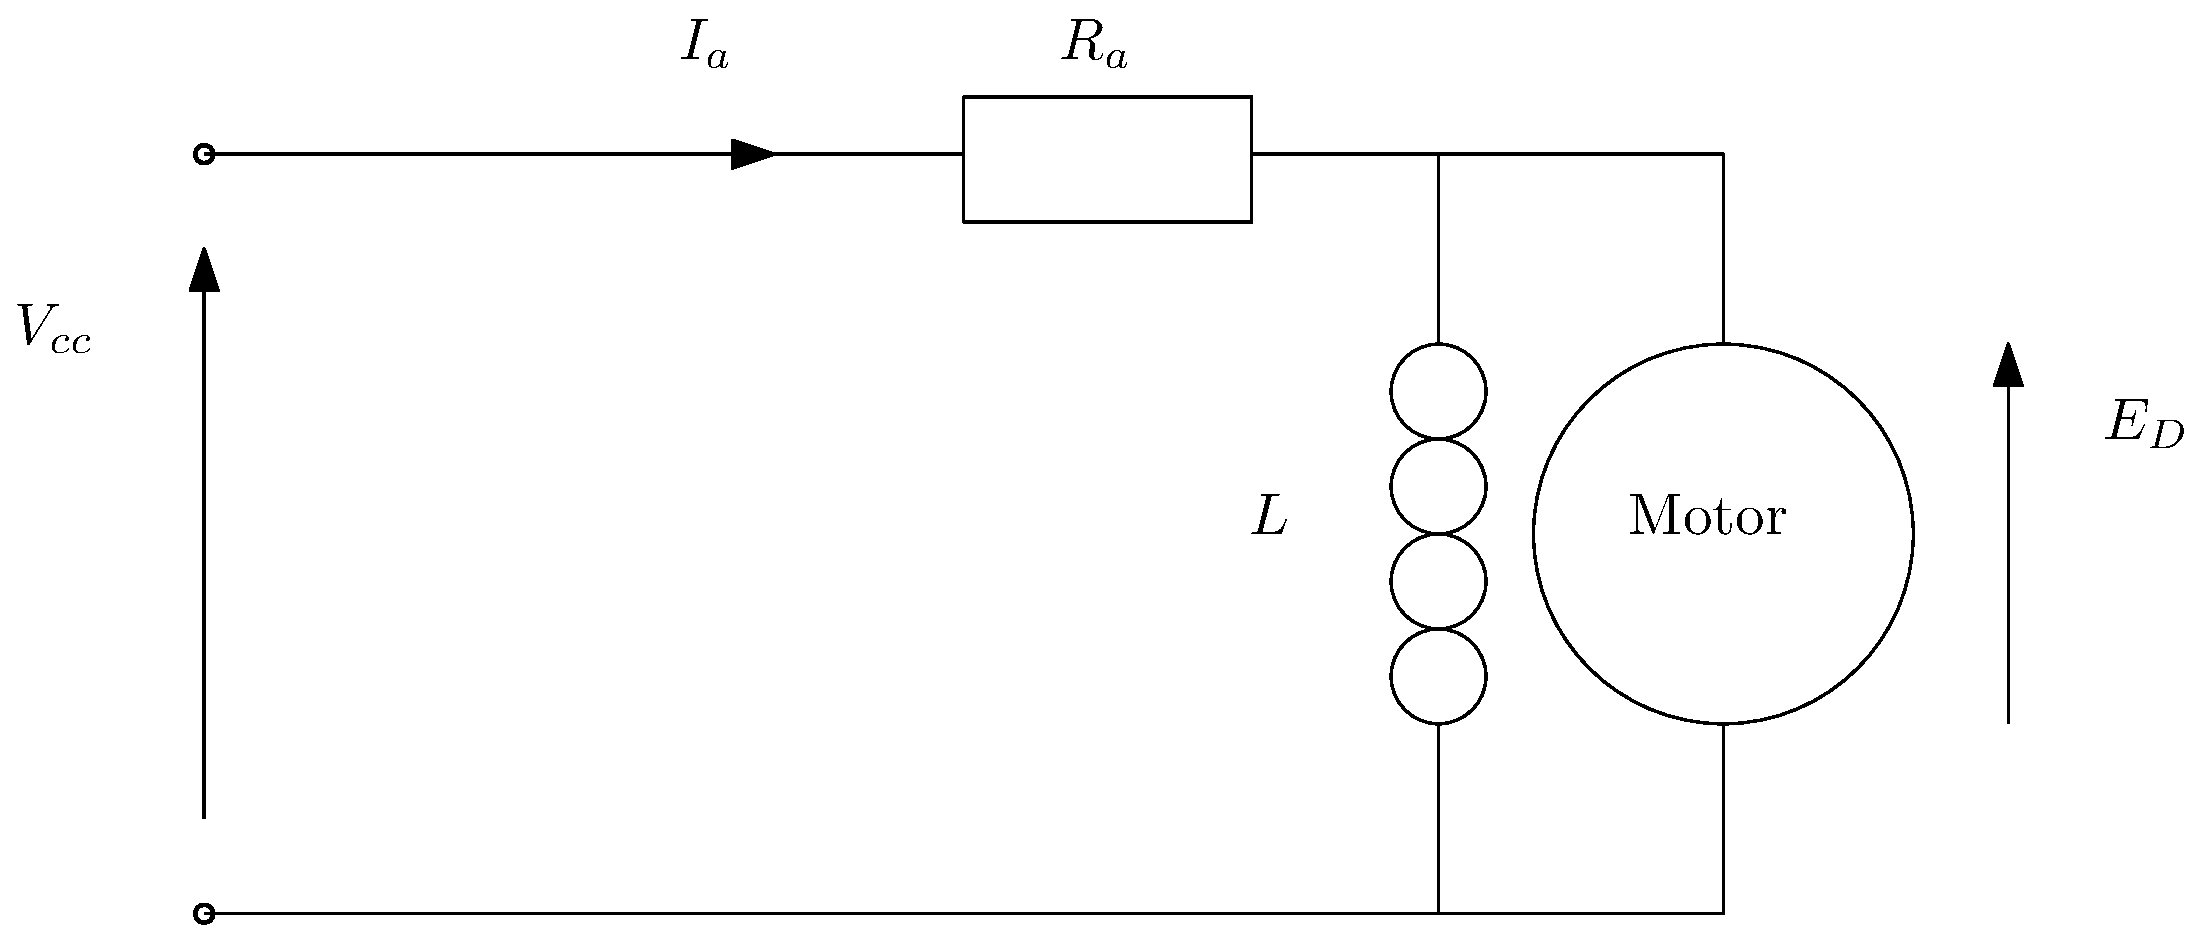
\includegraphics[width=0.9\linewidth]{dc_circuit.eps}
	\caption{Steady state equivalent circuit for a DC motor.}
	\label{fig:dc_circuit}
\end{figure}


 \begin{table}
 	\caption{Motor parameters used in simulation. Electric fork lift mass and speed \cite{Hyster2020a}. Motor and Electrical parameter from \cite{Racewicz2018}. *Computed for equivalent circuit in Equation \ref{eq:model} to match $\tau_{max}$ at $i_{max}$ }
 	\label{tab:motor_params} 
 	\centering
 	\begin{tabular}{ |c|c|c| }
 		\hline
 		$a_{max}$ & 2.5 & m/s$^2$\\
 		$v_{max}$ & 5.0& m/s \\
 		$k_v$ & 6 & rpm/V\\ 
 		$k_T$ & 1.53 & Nm/A\\ 
 		$P_{mech}@375$rpm & 3.6 & kW\\ 
 		$P_{elec}@375$rpm & 6.37 & kW \\
 		$\tau_{max}$ & 127.2 & Nm\\
 		*$R_a$ & 0.5 & Ohms\\
 		$V_{CC}$ & 72 & V\\
 		$i_{max}$ & 80 & A\\
 		$M$ & 400 & kg\\
 		$d_W$ & 0.256 & m\\
 		\hline
 	\end{tabular}
 \end{table}

As the top speed $v=5$m/s is quite low, and the vehicles stop and start frequently, air resistance which varies according to Equation \ref{eq:air_resistance} was found to be an order of magnitude smaller than the electrical losses, based on a frontal area $A=1$m$^2$ and the The drag coefficient $C$=1 for a cuboid shape was used, taken from \cite{Toolbox2004}. Air density is taken to be $\rho=1.224$kg/m$^2$.

\begin{equation}
F_a = C\rho A v^2 
\label{eq:air_resistance}
\end{equation}

A brushless DC motor for an industrial vehicle typically has a constant voltage from a battery pack \cite{Hyster2020a}. In this case we set $V_a=$72V, within the range tested in \cite{Racewicz2018}. Torque can be varied from zero to maximum by changing the slip angle between the magnetic field generated digitally by the three phase coils and the magnetic field generated by the hgh strength magnets fixed on  the rotor. The output of the vehicle's longitudinal speed controller must therefore be a duty cycle $-1.0<d<1.0$. A value of zero corresponds to zero torque, where the slip angle is zero, and a value of +/-1.0 to a slip angle of +/-90 degrees where torque is at a maximum in forward or reverse respectively.


\section{Method}
To examine control of variable numbers of vehicles, and comment on safety effects as well as performance of experimental algorithms utilizing a dynamic simulation test environment seemed prudent to start with. The goal here is to examine edge cases which are safety critical (may lead to a collision between AGV). The different algorithms will be compared based on execution time, total travel time, total energy consumption and mean throughput delay with a given traffic pattern.

\subsection{Conflict Zone Approximation}
\label{sec:conflict_zone}
The collision avoidance constraints are simplified by merging all the conflicts on each path, to keep only the smallest $s_B$ and the largest $s_C$ for that path. The extent of the conflict zone for vehicle$i$ is given by Equation \ref{eq:distance_threshold}. The conflicted segment of each vehicle's path lies between $s_B$ the smallest value of $s$ which satisfies Equation \ref{eq:distance_threshold} and $s_C$ the largest value. The union of these conflicted segments form the total conflict zone, which is an irregular non-convex, connected compound shape. 

In some cases it may be advantageous to limit mutual exclusion by only considering path segments which have different orientations to be in conflict, even if they satisfy Equation \ref{eq:distance_threshold}. This could allow closer spacing of AGV travelling in the same direction by following according to the distance measured to leader by on-board sensors.

\begin{equation}
\label{eq:distance_threshold}
||X_i(s) - X_j(t)|| < W_v \quad \forall j \in N, \quad j>i\\
\end{equation}

\subsection{Objective}
The objective to minimize the total travel time is given by Equation \ref{eq:objective}. It is linear terms of the reciprocal speed vector $\bm{\phi} \in R^{(n \times n)}$, which has up to two elements per AGV. One for the approach if it has not yet been passed and one for the conflict so $\bm{\phi}_i = [\phi_{AB}, \phi_{BC}]$. The segment lengths for the approach and the conflict are contained in distance vector $\bm{d}$ so $\bm{d}_i =[d_{AB}, d_{BC}] $.

\begin{equation}
\label{eq:objective}
\begin{array}{c}
\min \limits_{\bm{\phi}} \bm{J}_T = \bm{d}^T\bm{\phi} \\ 
$subject to$\\
\bm{\phi} > \phi_{min} \\
\bm{\phi}^T \bm{H_{ij}} \bm{\phi} > 0 \quad \forall i, j \in [1,p] \quad $with $ j > i \\
\end{array}
\end{equation}

The condition $j > i$ in Equation \ref{eq:objective} indicates that the number of constraints varies with the number of vehicles $p$ as $\frac{p(p-1)}{2}$. This corresponds to one constraint between each pair of approaching AGVs.

\subsection{Differential Constraints}
Vehicle acceleration limits are dealt with implicitly, by the maximum speed which can be expressed as a lower bound on $\bm{\phi} < \phi_{min}$. The simulated value $\phi_{min}$=5m/s, is reachable within a certain distance $d_{min}$ from any feasible starting speed, assuming a constant limited acceleration $a_{max}$ according to $v_{max} = \sqrt{2 a_{max} d_{min}} $. Using the parameters from Table \ref{tab:params}, the acceptable distance is $d_{min}=$5m.

\subsection{Online Feedback Considerations}
In order to guarantee feasibility we need only to ensure the conflict zone length $d_{BC}$ and the approach length $d_{AB}$ are both greater than $d_min$ when vehicles receive their instructions. A vehicle proceeding toward the conflict will eventually pass the point of no return where $d_{AB} = d_{min}$. It can not be guaranteed that any instructions sent after this point can be satisfied by the on-board longitudinal control. Any vehicle past the point of no return appears in the optimization as a constant constraint on the speeds of subsequent vehicles. The constraint uses the latest reported speed and position for real-time feedback, so if a vehicle past the point of no return fails to meet its deadline, the later vehicles can be safely delayed until it leaves the conflict zone.  

\subsection{Conflict-zone Collision Avoidance Constraints} 
By definition, each intersection controller is responsible for one conflict zone, constructed as explained in Section \ref{sec:conflict_zone}. This makes it
possible to express the constraint that vehicles do not collide
in terms of time. Vehicle $i$ arrives at the first conflicted
segment $\omega_min$ and departs from the last at $\omega_{max}$ . The following three subsections set out three alternative ways
of expressing the collision avoidance constraints which have
been evaluated. The arrival time is given by Equation \ref{eq:arrive}. Considering average speeds, the departure time $\omega_{max}$ is also linear, this is given by Equation \ref{eq:depart}.

\begin{equation}
\label{eq:arrive}
\omega_i^{min} = d_{AB} \phi_{AB} = \bm{e}^T \bm{\phi}_i
\end{equation}

Where
\begin{equation}
\label{eq:e_vec}
\bm{e}^T = [d_{AB}, 0]
\end{equation}
and 
\begin{equation}
\label{eq:depart}
\omega_i^{max} = [d_{AB}, d_{BC}]\left[\begin{array}{c}
\phi_{AB}\\
\phi_{BC}
\end{array}\right] = \bm{f}^T \bm{\phi}_i
\end{equation}
Where
\begin{equation}
\label{eq:f_vec}
\bm{f}^T = \begin{cases}
    [d_{AB}, d_{BC}],& \text{if } d_{AB}> 0\\
    [0, d_{BC}],              & \text{otherwise}
\end{cases}
\end{equation}

Following \cite{Digani2019}, the time window between $\omega_{min}$ and $\omega_{max}$ may be expressed in terms of the midpoint $\alpha$ and the extent $\beta$. In this way the collision avoidance constraints in Equation \ref{eq:mod_cons} are independent of the order in which AGV $i$ and AGV $j$ arrive.

\begin{equation}
\label{eq:mod_cons}
|\alpha_i - \alpha_j|> \beta_i + \beta_j
\end{equation}

Here
\begin{equation}
\alpha_i = \omega_i^{max} + \omega_i^{min}
\end{equation}
represents the midpoint of the time vehicle $i$ occupies the conflicted segment and and
\begin{equation}
\beta_i = \omega_i^{max} - \omega_i^{min}
\end{equation}
represents the range of the time either side of the midpoint, both scaled by a factor of two.

In matrix form this can be written
\begin{equation}
\label{eq:alpha_mat}
\alpha_i = \bm{f}^T\bm{\phi}_i + \bm{e}^T\bm{\phi}_i = \bm{1}_i^T\bm{A}\bm{\phi}_i
\end{equation}
with $\bm{A}= $ diag$(\bm{f} + \bm{e})$
\begin{equation}
\label{eq:beta_mat}
\beta_i = \bm{f}^T\bm{\phi}_i - \bm{e}^T\bm{\phi}_i = \bm{1}_i^T\bm{B}\bm{\phi}_i
\end{equation}
with $\bm{B}= $ diag$(\bm{f} - \bm{e})$

\subsection{Extra Constraint Between Vehicles in the Same Lane}
Vehicles travelling in the same lane forming a moving queue are more constrained than vehicles approaching a conflict zone. AGV are assumed here to be unable to overtake safely based on local sensors. This is likely to hold even with recent AGV which are capable of significant autonomy including adaptive path planning. This is because floor space is at a premium in a logistic environment so the gaps between the shelves are unlikely to be much wider than one AGV.

Indices are increasing so vehicle (i+1) is following behind vehicle (i). The safety constraint between vehicles in the same lane $l$ to ensure they remain a safe distance $L$ apart is given by Equation \ref{eq:in-lane1}
\begin{equation}
s_{i} > s_{i+1} + L \quad \forall i \in l
\label{eq:in-lane1}
\end{equation}
This can be expressed in terms of minimum time to collision of $TTC_{min} = 2 L/(v_i + v_{i+1})$ as in Equation \ref{eq:in-lane2}.
\begin{equation}
(s_{i}-s_{i+1})/(v_i - v_{i+1})) > TTC_{min}
\label{eq:in-lane2}
\end{equation}

It is a little awkward to capture this constraint exactly using the average speed on two segments. This approximation in Equation \ref{eq:in-lane3} was tested.
\begin{equation}
(s_{i}-s_{i+1})(\phi_i - \phi_{i+1})) > TTC_{min}
\label{eq:in-lane3}
\end{equation}  
\subsection{Non-Convex Quadratic Constraints Optimal Intersection Control}
\label{sec:quad}
Equation \ref{eq:mod_cons} can be converted to standard form by squaring both sides and substituting the matrix expressions for $\alpha_i$ and $\beta_i$. This gives the matrix inequality for each pair of vehicles shown in Equation \ref{eq:lambda}.
\begin{equation}
[\bm{\phi}_i^T, \bm{\phi}_j^T] \left[\begin{array}{cc}
\bm{\Lambda}_{ij}^{ii} & \bm{\Lambda}_{ij}^{ij} \\
\bm{\Lambda}_{ij}^{ji} & \bm{\Lambda}_{ij}^{jj}
\end{array}\right] > 0
\label{eq:lambda}
\end{equation}

The four pairwise submatrices can be expressed in terms of the diagonalized distance $\bm{A}$ and $\bm{B}$ as follows:
\begin{equation}
\bm{\Lambda}_{ij}^{ii} =  (\bm{A}_i - \bm{B}_i)\bm{1}_i\bm{1}_i^T(\bm{A}_i + \bm{B}_i)
\end{equation}

\begin{equation}
\bm{\Lambda}_{ij}^{jj} =  - (\bm{A}_j + \bm{B}_j)\bm{1}_j\bm{1}_j^T(\bm{A}_j + \bm{B}_j)
\end{equation}

\begin{equation}
\bm{\Lambda}_{ij}^{ij} = \bm{\Lambda}_{ij}^{ji T}  =  - (\bm{A}_j + \bm{B}_j)\bm{1}_j\bm{1}_i^T(\bm{A}_i + \bm{B}_i)
\end{equation}

For more than two vehicles this can be arranged into a
block diagonal matrix $\bm{H}_{ij} \in R^{(n \times n)}$ which is compatible with the input parameters, but still only represents the constraints between a pair with zeros for the other elements. The full constraint matrix $\bm{H}$ is the sum of these pairwise matrices, for every pair with $j<i$. 


%The intersection controller's task is to search over feasible speed profiles for the set which minimizes the total travel time for all approaching vehicles to cross the conflict zone. It was implemented following the description in \cite{Digani2019}, the only change being to express the constraints in path coordinates, rather than using discrete path segments, so they match up with the DualWaypoint interface and a fair comparison can be made with the other approaches.








\subsection{First-Come-First-Served Optimal Linear Intersection Control}
With a fixed ordering such as First-Come-First-Served, the reciprocal speed vector $\bm{\phi}$ is arranged in arrival order. 

The constraint in Equation \ref{eq:mod_cons} only needs to be applied between adjacent vehicles and it will hold for all vehicles. This reduces the number of constraints between $n$ vehicles to $n-1$.

The timing constraint that the leader exits the conflict zone before the follower enters is 
\begin{equation}
\omega_i^{max} > \omega_{i+1}^{min}
\end{equation}

This can be expressed as 
\begin{equation}
\bm{e}_i^T\bm{\phi}_i > \bm{f}_{i+1}^T\bm{\phi}_{i+1}
\end{equation}

leading to a pairwise matrix $Q^{ij} \in R^{(n \times n)}$
\begin{equation}
\bm{Q}^{ij}\bm{\phi} = \left[ \begin{array}{cccc}
0 & \hdots &&\\
\hdots & \bm{e}_i^T & -\bm{f}_{i+1}^T & \hdots \\
&&\hdots & 0\\
\end{array} \right]
\left[ \begin{array}{c}
\vdots\\
\bm{\phi}_i \\
\bm{\phi}_{i+1} \\
\vdots\\
\end{array} \right]
\end{equation}

The pairwise $Q^{ij}$ matrices are added together to get $A_{ub}$ in Equation \ref{eq:lin_cons}, 
\begin{equation}
\label{eq:lin_cons}
A_{ub}\bm{\phi} > 0
\end{equation}

The vehicles past the point of no return with latest feedback reciprocal speeds for each incomplete segment
\begin{equation}
\bm{p}_k  = [1/v_{AB}, 1/v_{BC}]
\end{equation}
are included in Equation \ref{eq:exit_constr} 
\begin{equation}
\bm{e}^T\bm{\phi}_i >  \bm{f}^T\bm{p}_k
\label{eq:exit_constr}
\end{equation} 
here $\bm{f}$ defined in Equation \ref{eq:f_vec}.
 
  
\subsection{Semaphore Based Collision Avoidance}
The constraints can be enforced without any optimization using a common synchronization object the binary semaphore. This is also based on first come-first-served ordering and the intersection controller gives the semaphore to the closest vehicle who provides an Approach Plan. This requires special messages in the dual waypoint interface, as the intersection controller makes no attempt to predict the time the conflict will become free. It issues a full speed ahead command to the vehicle with the semaphore and a space exclusion to all other vehicles. This consists of a distance along the AGVs submitted plan which it is not allowed to pass until given further instructions. 

This type of system is expected to lead to sub optimal throughput but be fast to calculate and guarantees safe operation. Similar schemes have been described in the literature so it is included in the comparison to give an idea of the benefits of departure time modelling and approach speed synchronization. 

\section{Numerical Results}

\begin{figure}[ht]
\centering
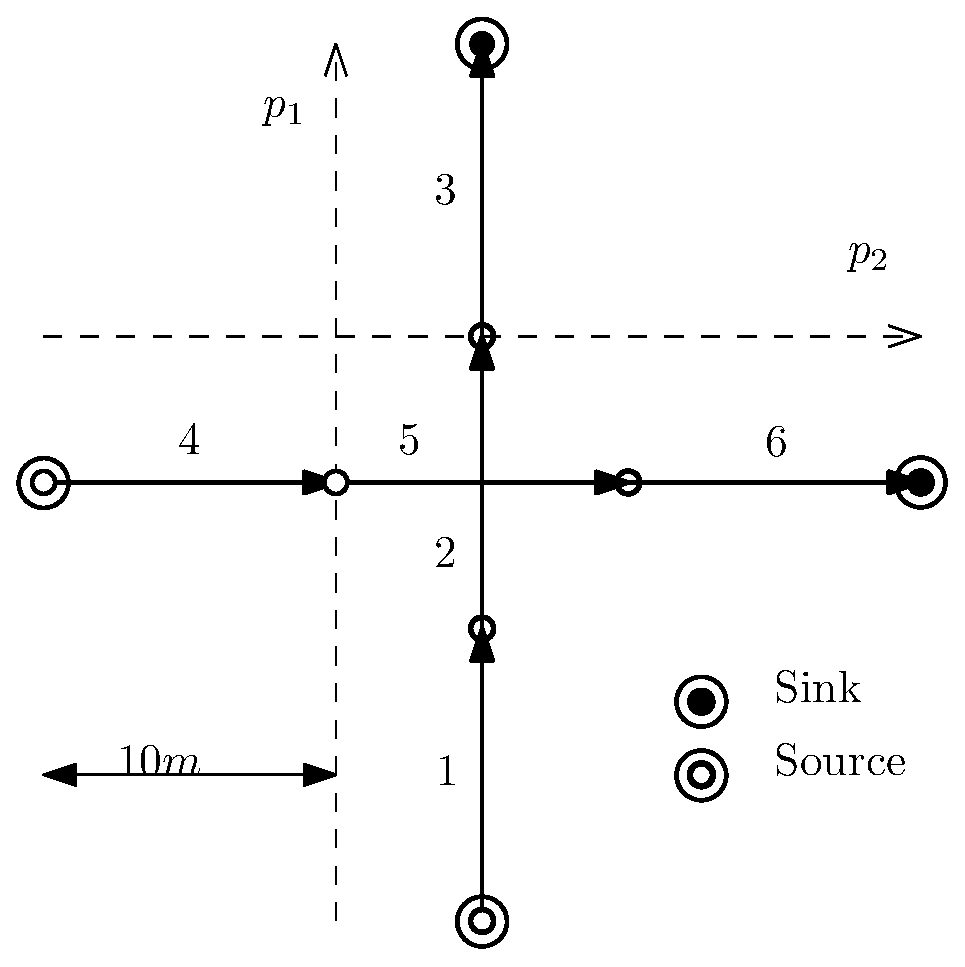
\includegraphics[width=0.9\linewidth]{intersection_topo}
\caption{Intersection layout with two conflicting routes.}
\label{fig:intersection_topo}
\end{figure}

The different approaches to intersection control were evaluated on a simulation of a simple intersection, comprised of two 30m lanes which cross in the middle as shown in Figure \ref{fig:intersection_topo}. There are two entrances to the map, one at the start of each lane. By varying the arrival rate $\lambda$ and the update frequency $f$, six scenarios were created with the parameters shown in Table \ref{tab:params}.
\begin{table}
\begin{tabular}{|c|c|c|c|}
\hline
	& $\lambda_1$ & $\lambda_2$ & $f$ \\
\hline
HLHT & 0.5 & 0.5 & 2 \\
HLMT & 0.1 & 0.5 & 2 \\
HLLT & 0.1 & 0.1 & 2 \\
LLHT & 0.5 & 0.5 & 10 \\
LLMT & 0.1 & 0.5 & 10 \\
LLLT & 0.1 & 0.1 & 10 \\
\hline
\end{tabular}
\label{tab:params}
\caption{Parameters for test scenarios. All units s$^-1$. }
\end{table}

Each scenario is identified with the first two characters relating to the latency between periodic messages from the intersection controller where High Latency is 500ms and  Low Latency is 100ms and the second two relating to the arrival rate, where High Traffic has $\lambda$=10 arrivals per second on both approaches, Low Traffic has $\lambda$=2 arrivals per second on both, and Mixed Traffic has one lane with $\lambda_1$=10 and the other with $\lambda_2$=2. For example High Latency, High Traffic becomes HLHT

\begin{table}
\begin{tabular}{|c|c|c|c|c|c|c|c|c|}
\hline
& T[s]&TTT[s]&t[s]&$\Delta$[s]&Ee[MJ]&Em[MJ]&Ex T[s]\\
\hline
FIFO & 45.7 & 181.0 & 6.033 & 0.033 & 43.906 & 30.323 & 0.0036\\
%FIFO HLMT & 70.9 & 181.5 & 6.05 & 0.05 & 52.225 & 35.083 \\
Quad & 44.8 &181.6& 6.0533 & 0.053 & 44.832 & 30.964 & 0.5252\\
%Quad HLMT & 70.9 & 181.5 & 6.05 & 0.05 & 52.225 & 35.083 \\
Sema & 83.9 & 326.4 & 10.88 & 4.88 & 159.1 & 68.140 & <0.001\\
\hline
\end{tabular}
\label{tab:results}
\caption{Intersection performance over 30 crossings with three different controllers for the HLHT scenario. }
\end{table}

The effects of the different controllers can be seen in the position time trace for 30 simulated crossings. The conflict zone is protects the intersection between the two lanes at s = 15m. Both lanes are collapsed onto one diagram, with $\times$ markers for vehicles travelling along the x axis and $\bigtriangleup$ markers for vehicles travelling along the y-axis. The controller is successful provided only one type of marker is present in the conflict zone at one time. All controller are safe, so the main comparison is how much the vehicles must slow down, shown by the gradient of the lines.  
\begin{figure}
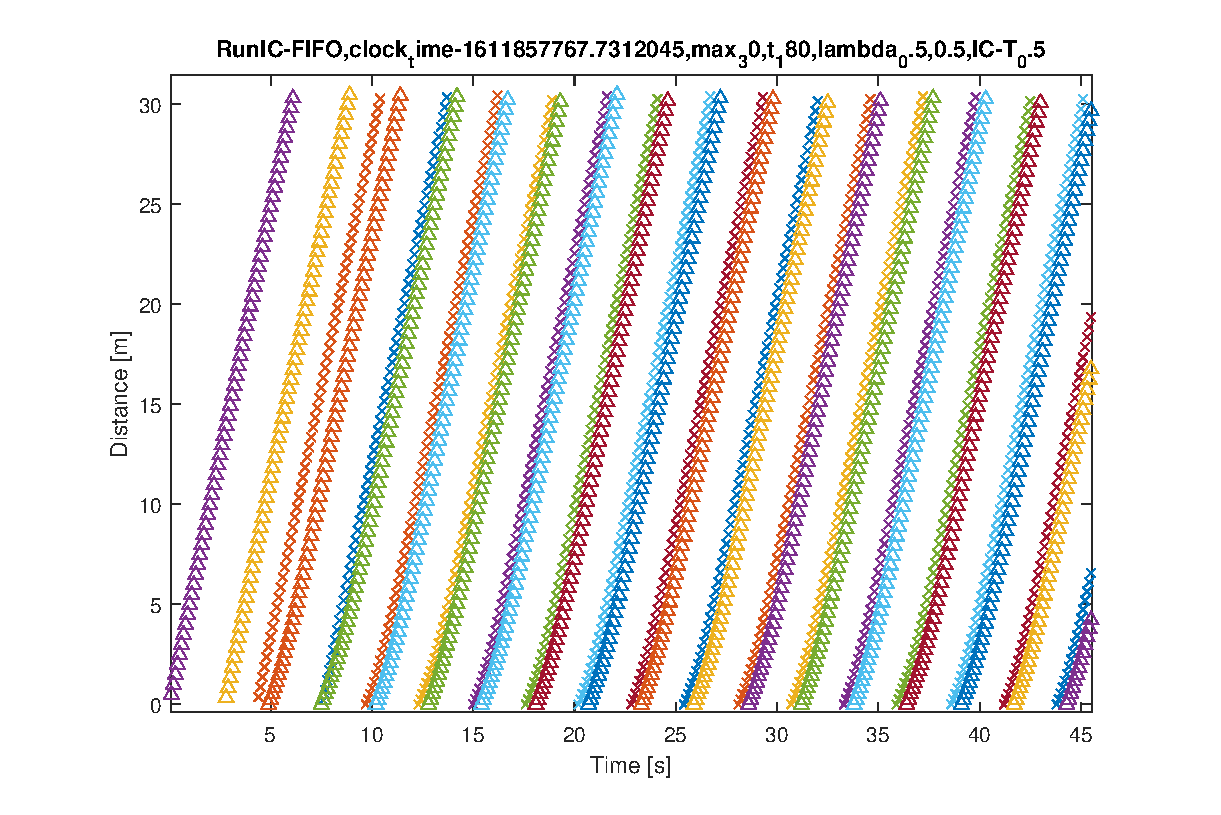
\includegraphics[width=1.0\linewidth]{results_fig/FIFO-HTHL_s-t.eps}
\label{fig:fifo_hlht}
\caption{Position-Time trace for HLHT Scenario under FIFO controller}
\end{figure}
\begin{figure}
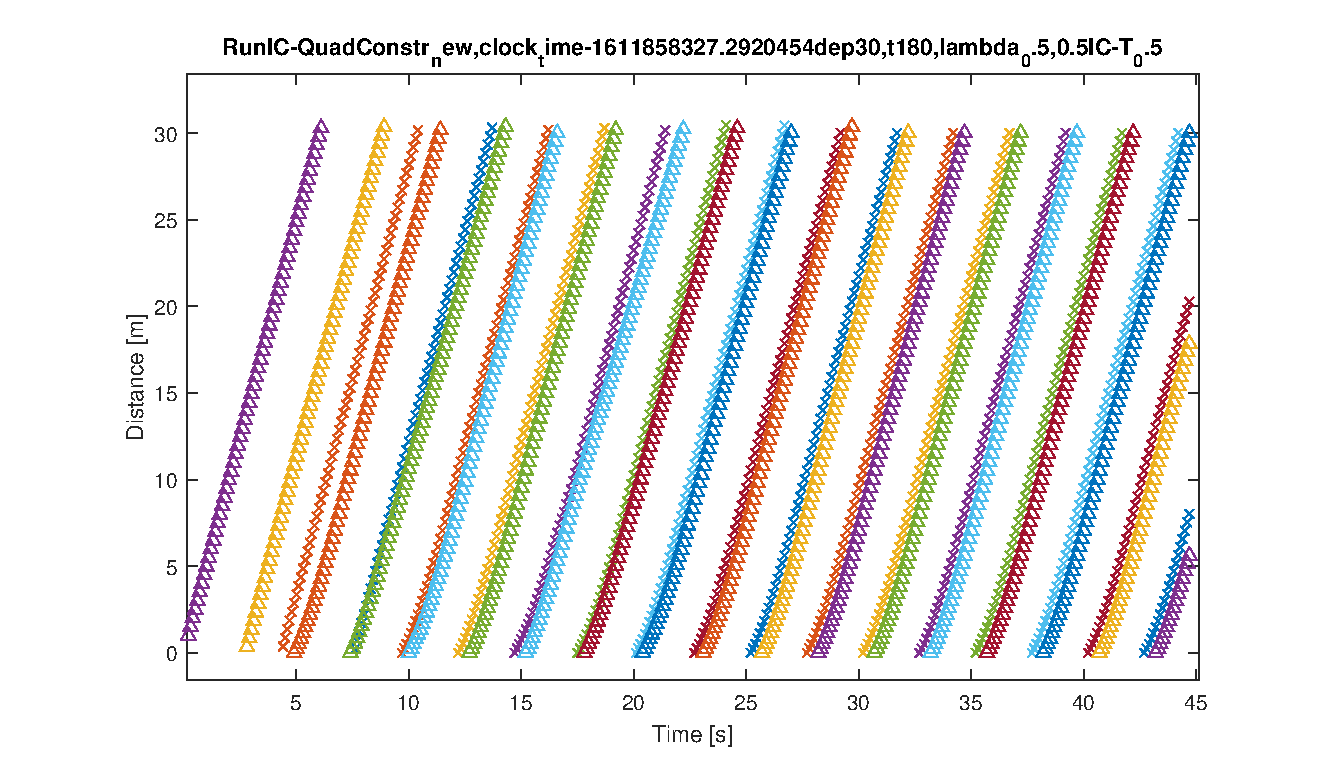
\includegraphics[width=1.0\linewidth]{results_fig/IC-QuadConstr_HLHT_s-t.eps}
\label{fig:quad_hlht}
\caption{Position-Time trace for HLHT Scenario under Quadratic Constraints controller}
\end{figure}
\begin{figure}
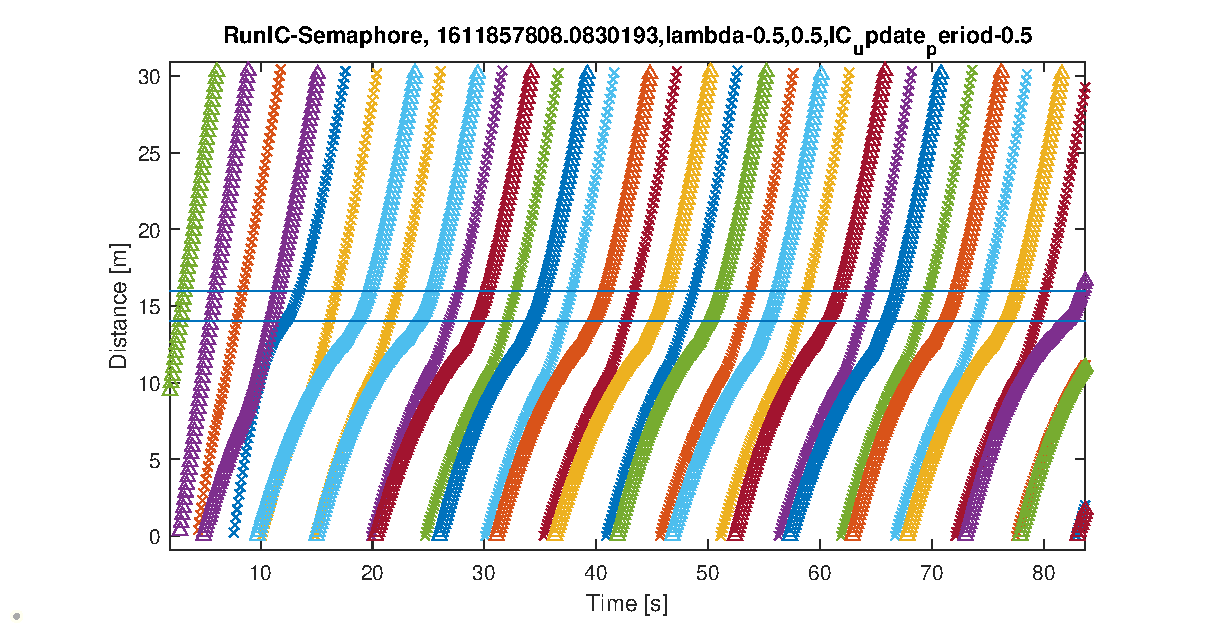
\includegraphics[width=1.0\linewidth]{results_fig/IC-Semaphore-HLHT.eps}
\label{fig:sema_hlht}
\caption{Position-Time trace for HLHT Scenario under Semaphore controller}
\end{figure}
The benefit of modelling the departure time and adjusting speeds in advance is clear from comparing the optimal controllers in Figure \ref{fig:fifo_hlht} and Figure \ref{fig:quad_hlht} with the Semaphore approach in Figure \ref{fig:sema_hlht}. This corresponds to a reduction in delay of 4.85 seconds per vehicle according to Table \ref{tab:results}. 

The two optimal methods are very close, with FIFO achieving a slight improvement in total travel time of 0.6 seconds, but a lower completion time by 0.9 seconds. This discrepancy may occur because the waiting time in the arrival queue is not counted in the total travel time, which should be addressed in further testing. It is more likely the Quadratic constraints achieved a slight improvement in throughput because of the freedom to vary the departure order. However, the departure order in Figure \ref{fig:quad_hlht} turns out to be close to FIFO anyway.

Another avenue of comparison is the energy usage. The semaphore method uses much more energy as the vehicles have to slow down more. Energy usage is not included in the objective for the optimal methods, so the question depends on whether higher average speeds or more acceleration lead to higher losses with our simple motor model.
\begin{figure}
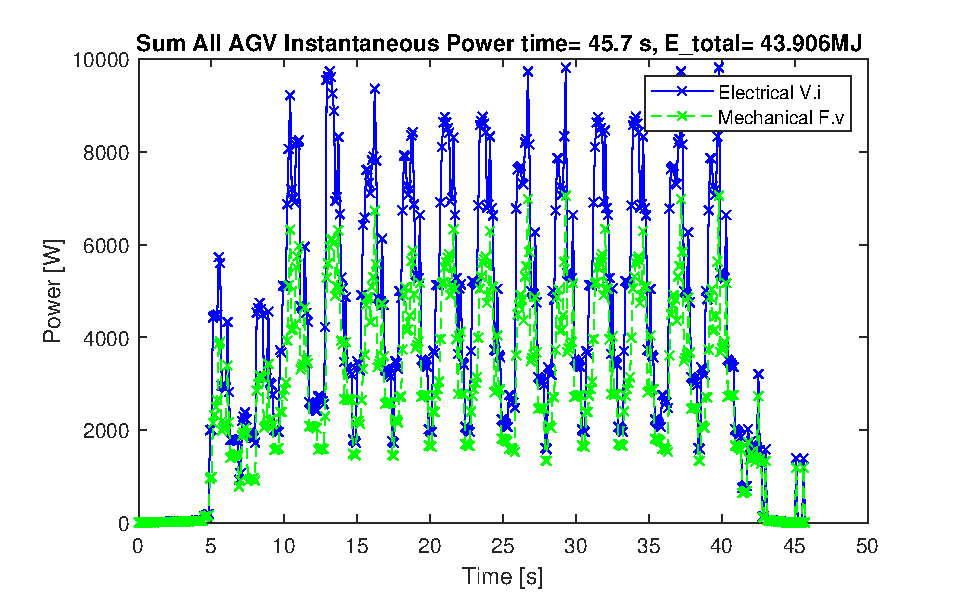
\includegraphics[width=1.0\linewidth]{results_fig/FIFO-HTHL_power_sum-t.eps}
\label{fig:fifo_hlht_pow}
\caption{Power Dissipation-Time trace for HLHT Scenario under FIFO controller}
\end{figure}
\begin{figure}
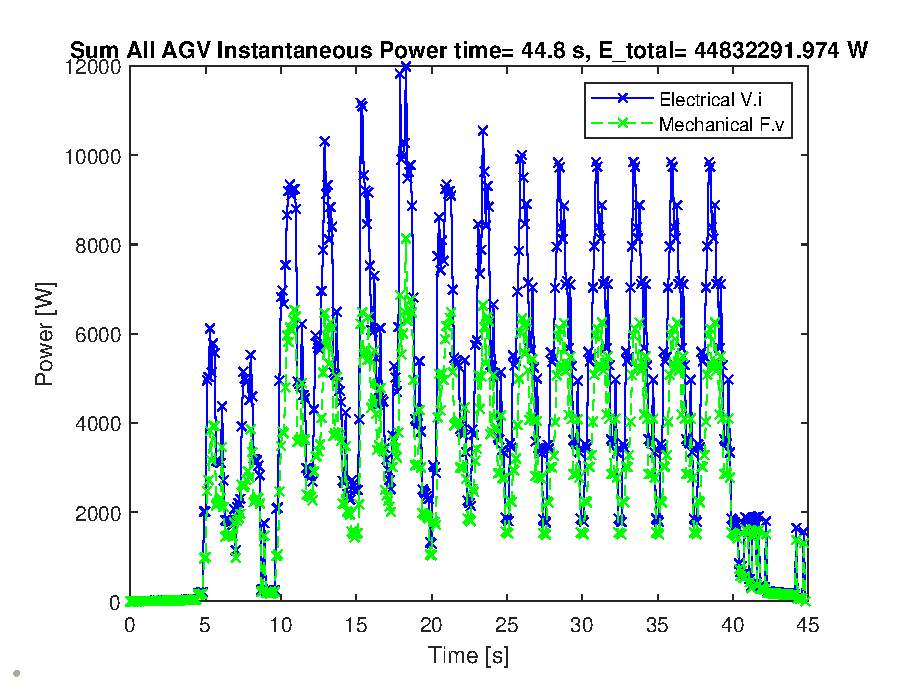
\includegraphics[width=1.0\linewidth]{results_fig/IC-QuadConstr_HLHT_powersum-t.eps}
\label{fig:quad_hlht_pow}
\caption{Power Dissipation-Time trace for HLHT Scenario under Quadratic Constraints controller}
\end{figure}
\begin{figure}
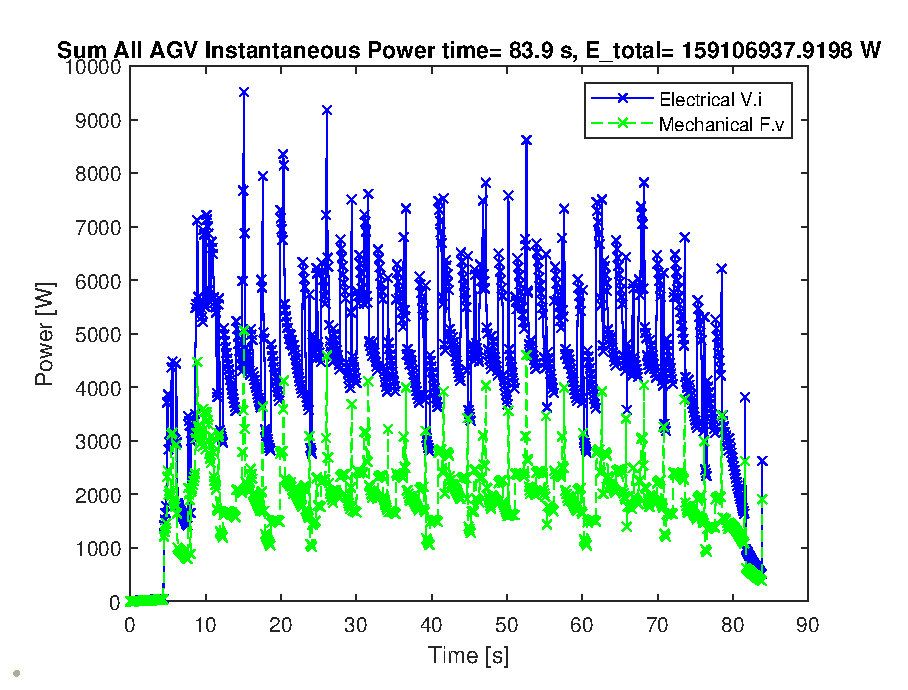
\includegraphics[width=1.0\linewidth]{results_fig/IC-Semaphore-HLHT-powersum.eps}
\label{fig:sema_hlht_pow}
\caption{Power Dissipation-Time trace for HLHT Scenario under Semaphore controller}
\end{figure}

The power consumption increase due to acceleration clearly dominates in Figure \ref{fig:sema_hlht_pow}, as the mechanical power is around 50 percent greater than in either of the optimal runs. This difference is compounded by the reduction in motor efficiency in high acceleration so the resultant increase in electrical poser dissipation is much greater, closer to 200 percent. 

There is still little to distinguish the two optimal approaches. Although unlike the delay, in this case maintaining FIFO order leads to a slight improvement: 43.9 MJ total energy compared to 44.8MJ. A spike in usage at around 18 seconds can be seen in Figure \ref{fig:quad_hlht_pow}, possibly this corresponds to a change in order which leads to lower delay but uses some extra energy. 


\subsection{Impact of Analytical Hessian on Execution Time of Trust Region Method}
The optimization problem with quadratic constraints described in Section \ref{sec:quad} was implemented in Python and solved periodically based on the latest position information at the specified control frequency $f$. The method chosen was 'trust-constr' from the Scipy.Optimize library \cite{scipy}. Trust region methods make use of the exact Semi-Definite Program relaxation for the Trust Region Sub-problem (TRS), of optimizing a non-convex quadratic objective subject to a Euclidean ball constraint, to iteratively solve general non-convex function with non-convex constraints by successive approximation\cite{conn2000trust}. They are likely to be more effective when the general problem has more in common with the TRS and recent methods have been proven to solve variants of that problem in linear time in terms of the input \cite{Wang2019}. Unlike some other general constrained optimization methods in Scipy.Optimize such as SLSQP, 'trust-constr' can make use of the analytical Hessian for the objective and constraints which may be important to exploit the linear objective and quadratic constraints.   

The Hessian must be provided to SciPy.Optimize in the form of a linear combination rather than a stacked matrix. This is to avoid forming the complete Hessian $H \in R^{(n \times np)}$ which may use a significant amount of memory for large problems. Instead, the analytical Hessian function must accept an additional parameter $v \in R^{(1 \times p)}$. This is a vector the same length as the constraints $c_{ineq} \in R^{(1 \times p)}$. The Hessian is returned as a $R^{(n \times n)}$, the weighted sum of pairwise blocks scaled according to $\sum_{i=1}^p v_i H_ij$.
  
With the analytical Hessian the average execution time for the Quadratic Constraints method over the HLHT run in which 30 vehicles passed through the intersection was 0.5251 seconds, varying between 0.0512 seconds to 1.215 seconds as the number of constraints varied from 1 to 6. Without the analytical Hessian of the constraints
Without the analytical constraint  Hessian the mean time taken over the same run was 0.383 seconds, varying between 0.0468 seconds to 7.696 seconds. It is surprising that the worst case time is so much worse and yet the mean time is better. This suggests that in the test data there are more cases with few constraints. It also motivates investigation into the cause of the outlier time. 

The execution time with the FIFO controller never exceeds 15.6 milliseconds on the same set of problems, with the average being 3.6 milliseconds. 

\section{Conclusion}
The advantages of centralized intersection optimization shown by previous authors are supported by our results.  Furthermore we show that enforcing first-in-first-out ordering leads to very similar performance in both delay and energy consumption on a simple intersection comprising two crossed lanes. For this reason the FIFO controller is a promising choice for real world implementation, as it can be solved orders of magnitude faster and captures almost all of the throughput advantage. The next step is to ensure this result holds for more complex intersections, where exploring alternative orderings may be more significant to the objective.    